%%%%%%%%%%%%%%%%%%%%%%%%%%%%%%%%%%%%%%%%%
% Beamer Presentation
% LaTeX Template
% Version 1.0 (10/11/12)
%
% This template has been downloaded from:
% http://www.LaTeXTemplates.com
%
% License:
% CC BY-NC-SA 3.0 (http://creativecommons.org/licenses/by-nc-sa/3.0/)
%
%%%%%%%%%%%%%%%%%%%%%%%%%%%%%%%%%%%%%%%%%

%----------------------------------------------------------------------------------------
%	PACKAGES AND THEMES
%----------------------------------------------------------------------------------------


\documentclass{beamer}

\mode<presentation> {
\usetheme{Madrid}

\setbeamertemplate{footline}[page number] % To replace the footer line in all slides with a simple slide count uncomment this line
\setbeamertemplate{navigation symbols}{} % To remove the navigation symbols from the bottom of all slides uncomment this line
}

\usepackage{graphicx}
\usepackage{booktabs}
\usepackage[T1]{fontenc}
\usepackage{amsmath}
\usepackage{mathtools}
\usepackage{amssymb}
\usepackage{graphicx}
\usepackage{graphics}
\usepackage{algorithmic}
\usepackage{algorithm}
\usepackage{listings}
\graphicspath{ {pictures/} }

\lstset{
	basicstyle=\footnotesize,
	tabsize=3,
}
%----------------------------------------------------------------------------------------
%	TITLE PAGE
%----------------------------------------------------------------------------------------

%\title[Short title]{Full Title of the Talk} % The short title appears at the bottom of every slide, the full title is only on the title page
\title[]{Theorem proving in Lean} % The short title appears at the bottom of every slide, the full title is only on the title page

\author{Mat\'u\v{s} Behun} % Your name
\institute[STU] % Your institution as it will appear on the bottom of every slide, may be shorthand to save space
{
Slovak University of Technology in Bratislava \\ % Your institution for the title page
\medskip
%\textit{john@smith.com} % Your email address
}
\date{\today} % Date, can be changed to a custom date

\begin{document}
%------------------------------------------------
\begin{frame}
\titlepage 
\end{frame}
%------------------------------------------------
%\begin{frame}
%\frametitle{Overview}
%\tableofcontents
%\end{frame}
%------------------------------------------------
% Introduction
%------------------------------------------------
\section{Computer proofs}
%------------------------------------------------
% Role of computers in theorem proving. It started with checking cases which
% were infeasable to check by hand in this case 1946 configurations,
% partly checked by hand. This was specialized software. Later proved by general
% purpose prover. At the begining help with proof by exhaustion.
%------------------------------------------------
\begin{frame}
    \frametitle{Computer aided proofs}
    Proving mathematical statements, showing that assumptions lead to the
    conclusion with help of automation.
    \begin{block}{Four color theorem}
        Plane divided into regions can be colored using 4-colors in  such a way
        that no boundary share same color.
    \end{block}
    After many attempts proved (1976) partially with help of computer. 1946
    configurations were checked by computer.
\end{frame}
%------------------------------------------------
% Automated theorem provers is topic in computer science. Most of these proofs
% are long and hard to prove. Problem with readability of output.
%------------------------------------------------
\begin{frame}
    \frametitle{Proof assistants}
    Software which requires human interaction during the process. Output has to
    be readable for human to make decision what to do next.
    \begin{itemize}
        \item Lean(2013) \\
        \item HOL - Higher Order Logic(1988) \\
        \item Coq(1989)
    \end{itemize}
    Why should we use proof assistants?
    \begin{itemize}
        \item Some mathematical fields more prone to make mistake \\
        \item Shinichi Mochizuki proving abc conjecture \\
    \end{itemize}
\end{frame}
%------------------------------------------------
% Curry-Howard correnspondence
%------------------------------------------------
\begin{frame}
    \frametitle{Curry-Howard correspondence}
    Establishes relation between formulas and proofs of those formulas in
    propositional intuitionistic logic and functions of a given type in a
    functional programming language. \\
    \begin{center}
        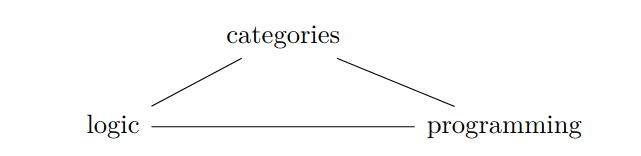
\includegraphics[width=0.5\textwidth]{three_way.png}
    \end{center}
    \color{black}\rule{\linewidth}{1pt}
    \begin{columns}[T]
        \begin{column}{.48\textwidth}
            First order logic formulas
            \begin{itemize}
                \item Variables called Terms \\
                \item Relations $\Rightarrow, \wedge, \vee, \dots$  \\
            \end{itemize}
        \end{column}
        \hfill
        \begin{column}{.48\textwidth}
            Sets
            \begin{itemize}
                \item Arbitrary elements
            \end{itemize}
        \end{column}
    \end{columns}
\end{frame}
%------------------------------------------------
% Curry-Howard correnspondence
%------------------------------------------------
\begin{frame}
    \frametitle{Curry-howard correspondence}
    \begin{columns}[T]
        \begin{column}{.2\textwidth}
        Predicate logic
        \end{column}
        \hfill
        \begin{column}{.48\textwidth}
        Sets
        \end{column}
    \end{columns}
    \color{black}\rule{\linewidth}{1pt}
    \begin{columns}[T]
        \begin{column}{.2\textwidth}
            \begin{itemize}
                \item $ p \wedge q $ \\
                \item $ p \vee q $
            \end{itemize}
        \end{column}
        \hfill
        \begin{column}{.6\textwidth}
            \begin{itemize}
                \item $ P \times Q = \{ (p, q) | p \in P$ and $q \in Q \} $ \\
                \item $ P \oplus Q = $ \\
            \end{itemize}
            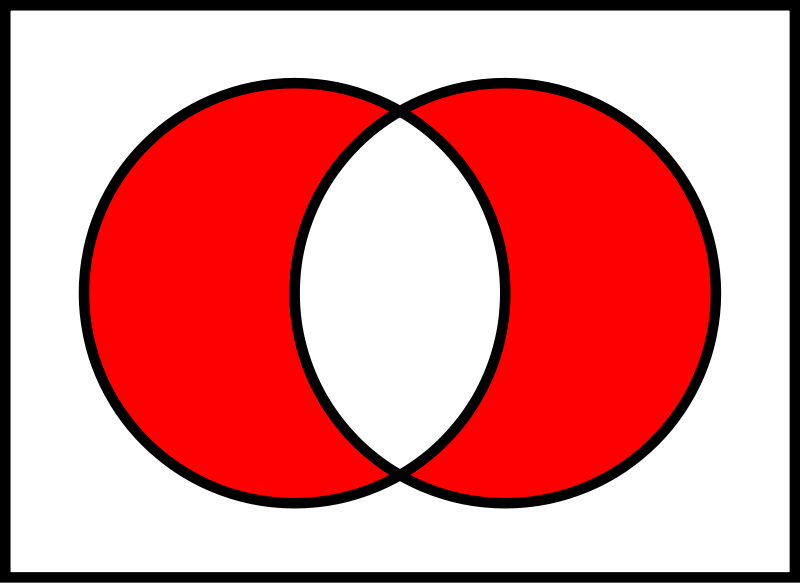
\includegraphics[width=0.5\textwidth]{exclusiveOr.png}
        \end{column}
    \end{columns}
\end{frame}
%------------------------------------------------
% Curry-Howard correnspondence
%------------------------------------------------
\begin{frame}
    \frametitle{Curry-howard correspondence}
    \begin{columns}[T]
        \begin{column}{.48\textwidth}
        Predicate logic
        \end{column}
        \hfill
        \begin{column}{.48\textwidth}
        Sets
        \end{column}
    \end{columns}
    \color{black}\rule{\linewidth}{1pt}
    \begin{columns}[T]
        \begin{column}{.48\textwidth}
            \begin{itemize}
                \item $ p \Rightarrow q $ \\
                \item $ \neg p $
            \end{itemize}
            \begin{displaymath}
                \begin{array}{|c c|c|}
                    p & q & p \Rightarrow q \\
                    \hline
                    T & T & T \\
                    T & F & F \\
                    F & T & T \\
                    F & F & T \\
                \end{array}
            \end{displaymath}
        \end{column}
        \hfill
        \begin{column}{.48\textwidth}
            \begin{itemize}
                \item $ P^{Q} \Leftrightarrow [ P, Q ]$ \\
                \item $ P^{\emptyset} $ \\
            \end{itemize}
        \end{column}
    \end{columns}
\end{frame}
%------------------------------------------------
% Curry-Howard correnspondence
%------------------------------------------------
\begin{frame}
    \frametitle{Curry-howard correspondence}
    \begin{columns}[T]
        \begin{column}{.48\textwidth}
        Predicate logic
        \end{column}
        \hfill
        \begin{column}{.48\textwidth}
        Sets
        \end{column}
    \end{columns}
    \color{black}\rule{\linewidth}{1pt}
    \begin{columns}[T]
        \begin{column}{.48\textwidth}
            \begin{itemize}
                \item $ p \wedge q \Rightarrow q $ \\
            \end{itemize}
        \end{column}
        \hfill
        \begin{column}{.48\textwidth}
            \begin{itemize}
                \item $ [ P \times Q, Q ] $
            \end{itemize}
        \end{column}
    \end{columns}
\end{frame}
%------------------------------------------------
% Lean
%------------------------------------------------
\begin{frame}
    \frametitle{Lean theorem prover}
    \begin{itemize}
        \item Functional programming language
        \item Interactive theorem prover
        \item Open source project backed by Microsoft Research
    \end{itemize}
\end{frame}
%------------------------------------------------
% Lean - motivation
%------------------------------------------------
\begin{frame}
    \frametitle{Why Lean}
    \begin{itemize}
        \item Able to make sophisticated objects - Perfectoid spaces
        \item used by XENA project, get mathematicians to use proof verification software
        \item mathlib(volunteering library of mathematics)
        \item active community
    \end{itemize}
\end{frame}
%------------------------------------------------
% Lean
%------------------------------------------------
\begin{frame}
    \frametitle{Lean enviroment}
    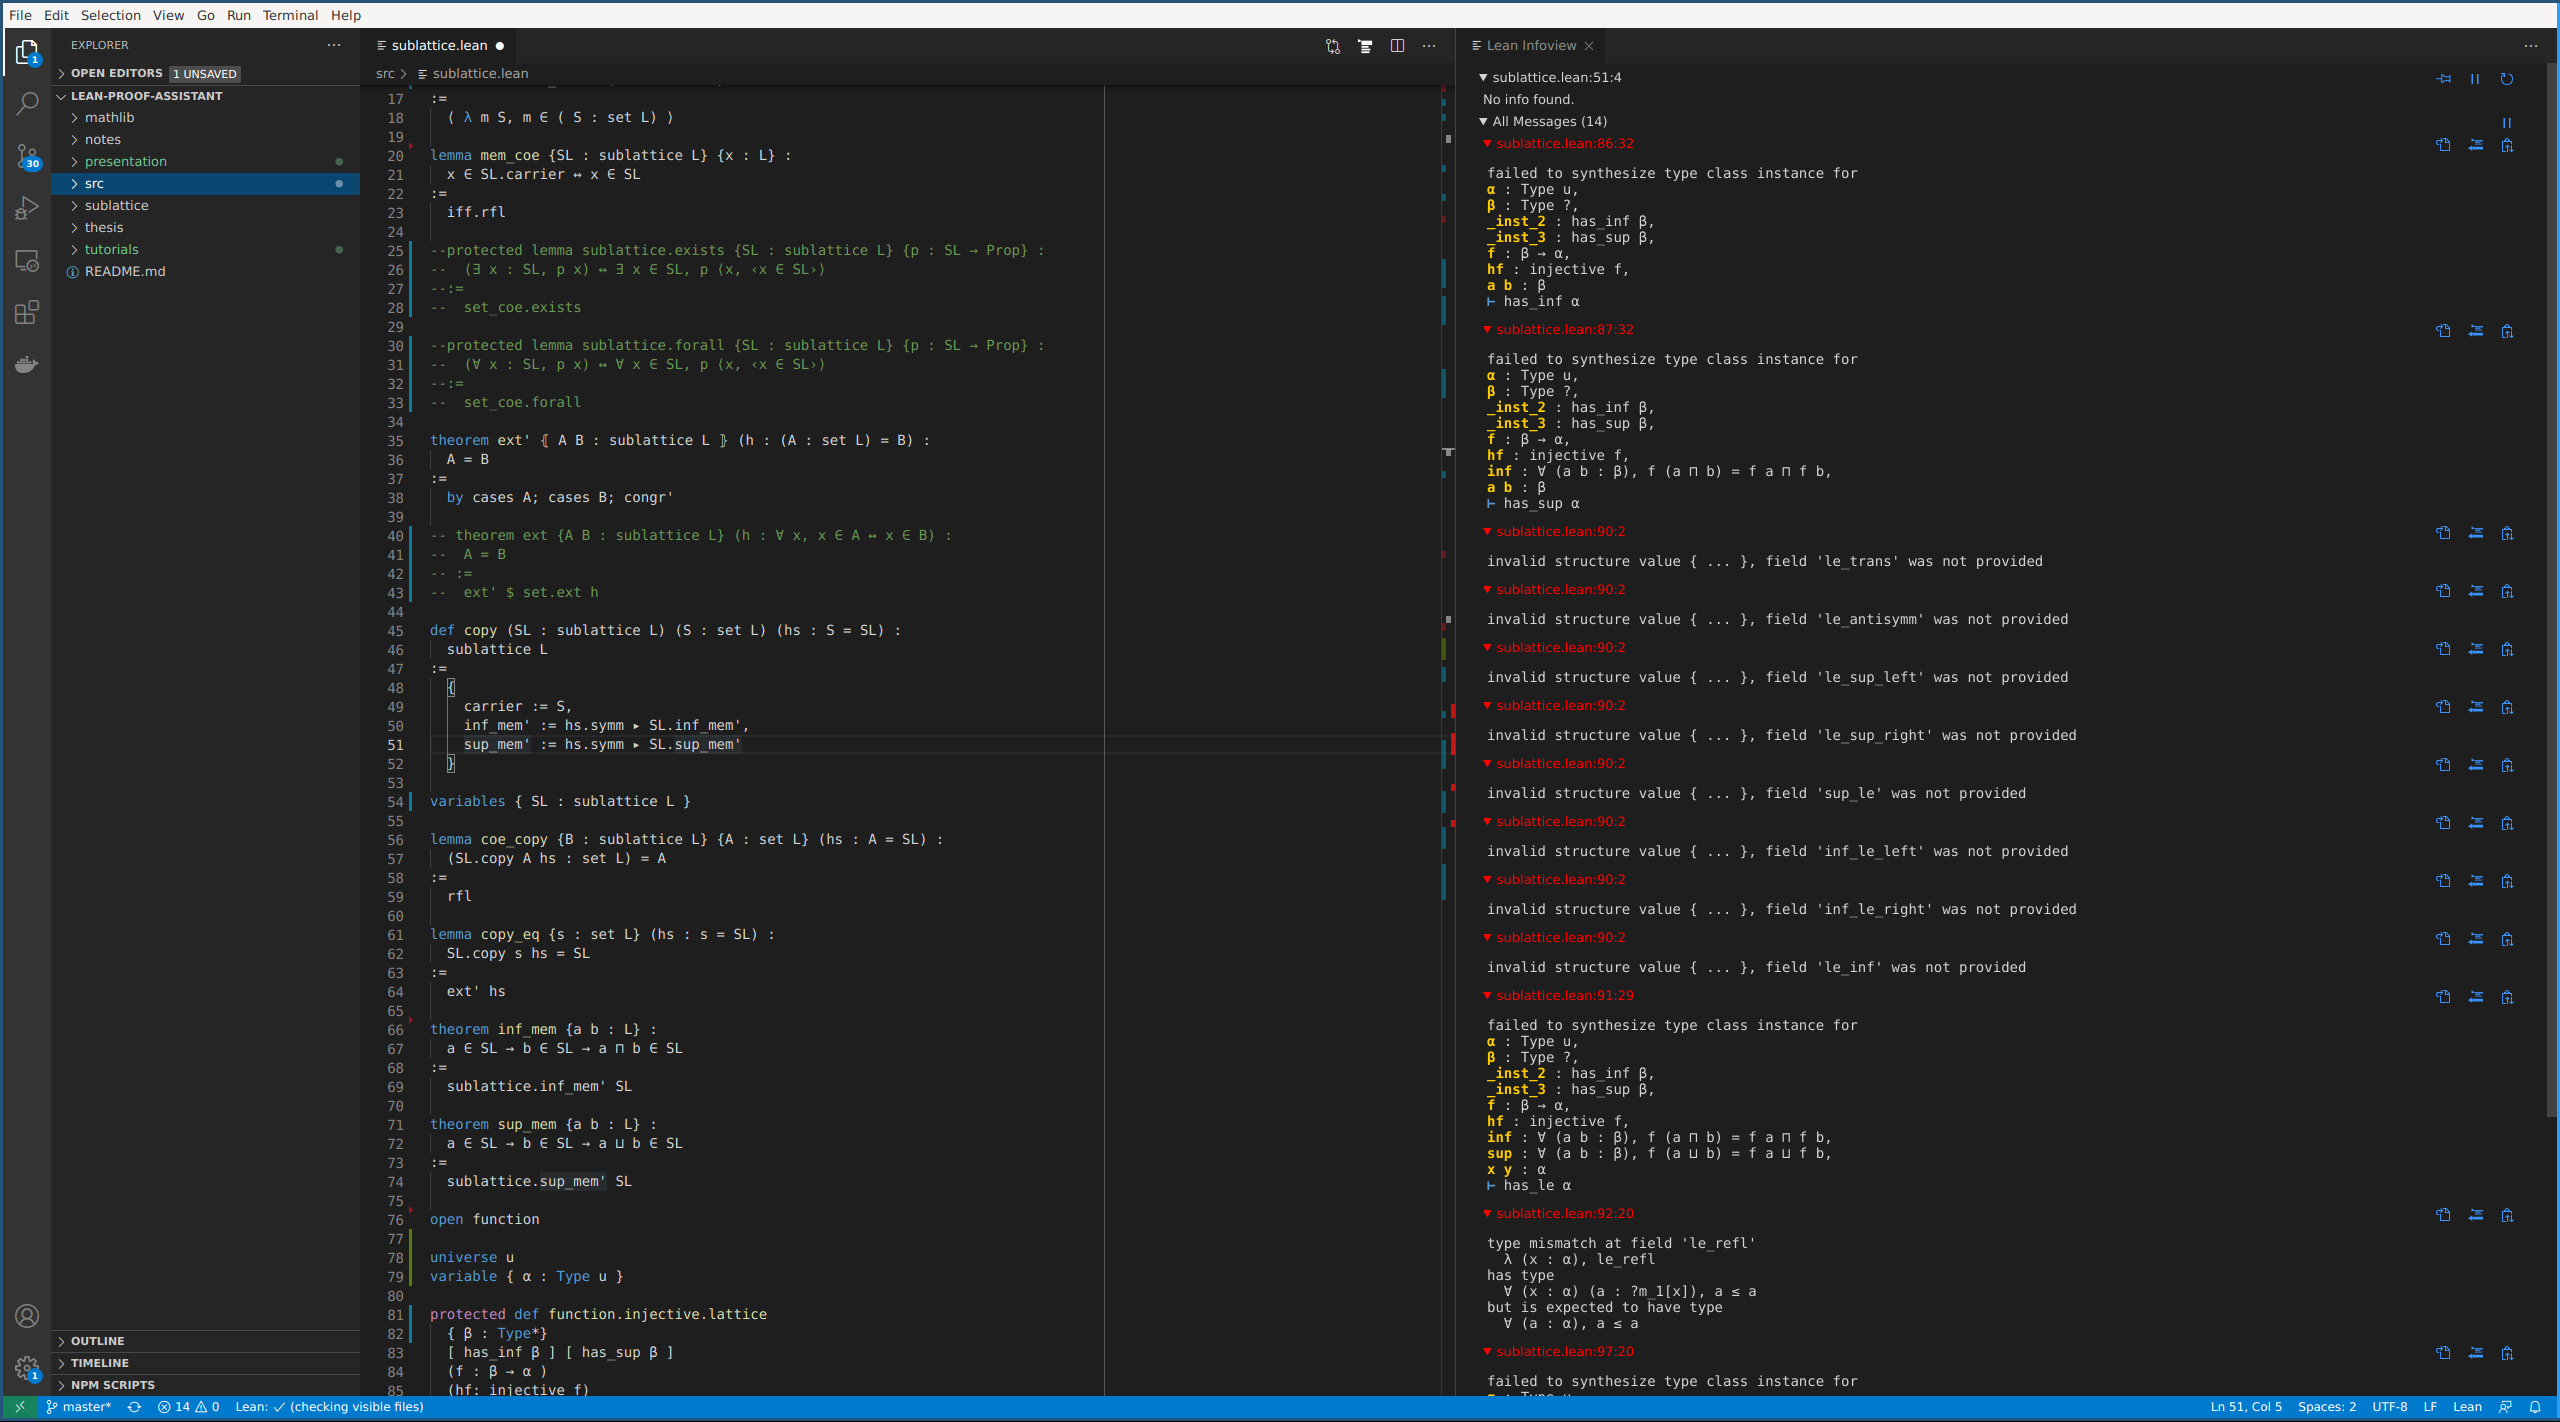
\includegraphics[width=1\textwidth]{code_sublattice.png}
\end{frame}
%------------------------------------------------
% Forward proving
%------------------------------------------------
\begin{frame}
    \frametitle{Forward proving}
    Two types of proving in Lean forward, backwards
    \texttt{
        \begin{tabbing}
            variables p q : Prop \\
            \\
            theorem t1 : \\
            p $\to$ q $\to$ p \\
            := \\
            $\lambda$ (hp : p), $\lambda$ (hq : q), hp \\
        \end{tabbing}
    }
\end{frame}
%------------------------------------------------
% Backward proving
%------------------------------------------------
\begin{frame}
    \frametitle{Backwards proving - using tactics}
    \texttt{
        \begin{tabbing}
            variables p q : Prop \\
            \\
            theorem t2 : \\ 
            Q $\to$ (P $\vee$ Q) \\
            := \\
            begin \\
            intro a, \\
            right, \\
            exact a, \\
            end \\
        \end{tabbing}
    }
\end{frame}
\begin{frame}
    \frametitle{Backwards proving - usings tactics}
    \texttt{
        \begin{tabbing}
            import algebra.group.defs \\
            \\
            variables (G : Type*) [group G] (a b c : G) \\
            \\
            theorem t3 : $a * a^{-1} * 1 * b = b * c * c^{-1}$ \\
            := \\
            begin \\
              simp \\
            end
        \end{tabbing}
    }
\end{frame}
\begin{frame}
    \frametitle{What else...}
    \begin{itemize}
        \item Get contribution to mathlib
        \item Better explanation of type theory and structures
    \end{itemize}
\end{frame}
\begin{frame}
    \frametitle{Thank you for your attention}
    \begin{itemize}
        \item author = Samuel Mimram,
        \item title = PROGRAM = PROOF,
        \item publisher = Independently published,
        \item year = 2020,
        \item isbn = 979-8615591839,
    \end{itemize}
    \color{black}\rule{\linewidth}{1pt}
    \begin{itemize}
        \item https://leanprover.github.io/theorem \\
            \_proving\_in\_lean/introduction.html
    \end{itemize}
    \color{black}\rule{\linewidth}{1pt}
    \begin{itemize}
        \item http://wwwf.imperial.ac.uk/~buzzard/xena/natural\_number\_game/
    \end{itemize}
\end{frame}
\end{document}
